\documentclass[12pt,a4paper]{article}

\usepackage[utf8]{inputenc}
\usepackage[T2A]{fontenc}
\usepackage[ukrainian]{babel}

\usepackage{geometry}
\geometry{left=2cm,right=2cm,top=2cm,bottom=2cm}

\usepackage{graphicx}
\usepackage{array,multirow}
\usepackage{booktabs}
\usepackage{caption}
\usepackage{subcaption}
\renewcommand{\thetable}{№\arabic{table}}
\captionsetup[table]{name=Таблиця}
\captionsetup[subfigure]{labelformat=simple,labelsep=space}

\usepackage{amsmath}
\usepackage{pdflscape}
\usepackage{xcolor}

\usepackage{hyperref}

\renewcommand\thesubfigure{(\alph{subfigure})}

\begin{document}

    \begin{titlepage}

        % Картинка шапки (по центру, з відступом від верху)
        \begin{center}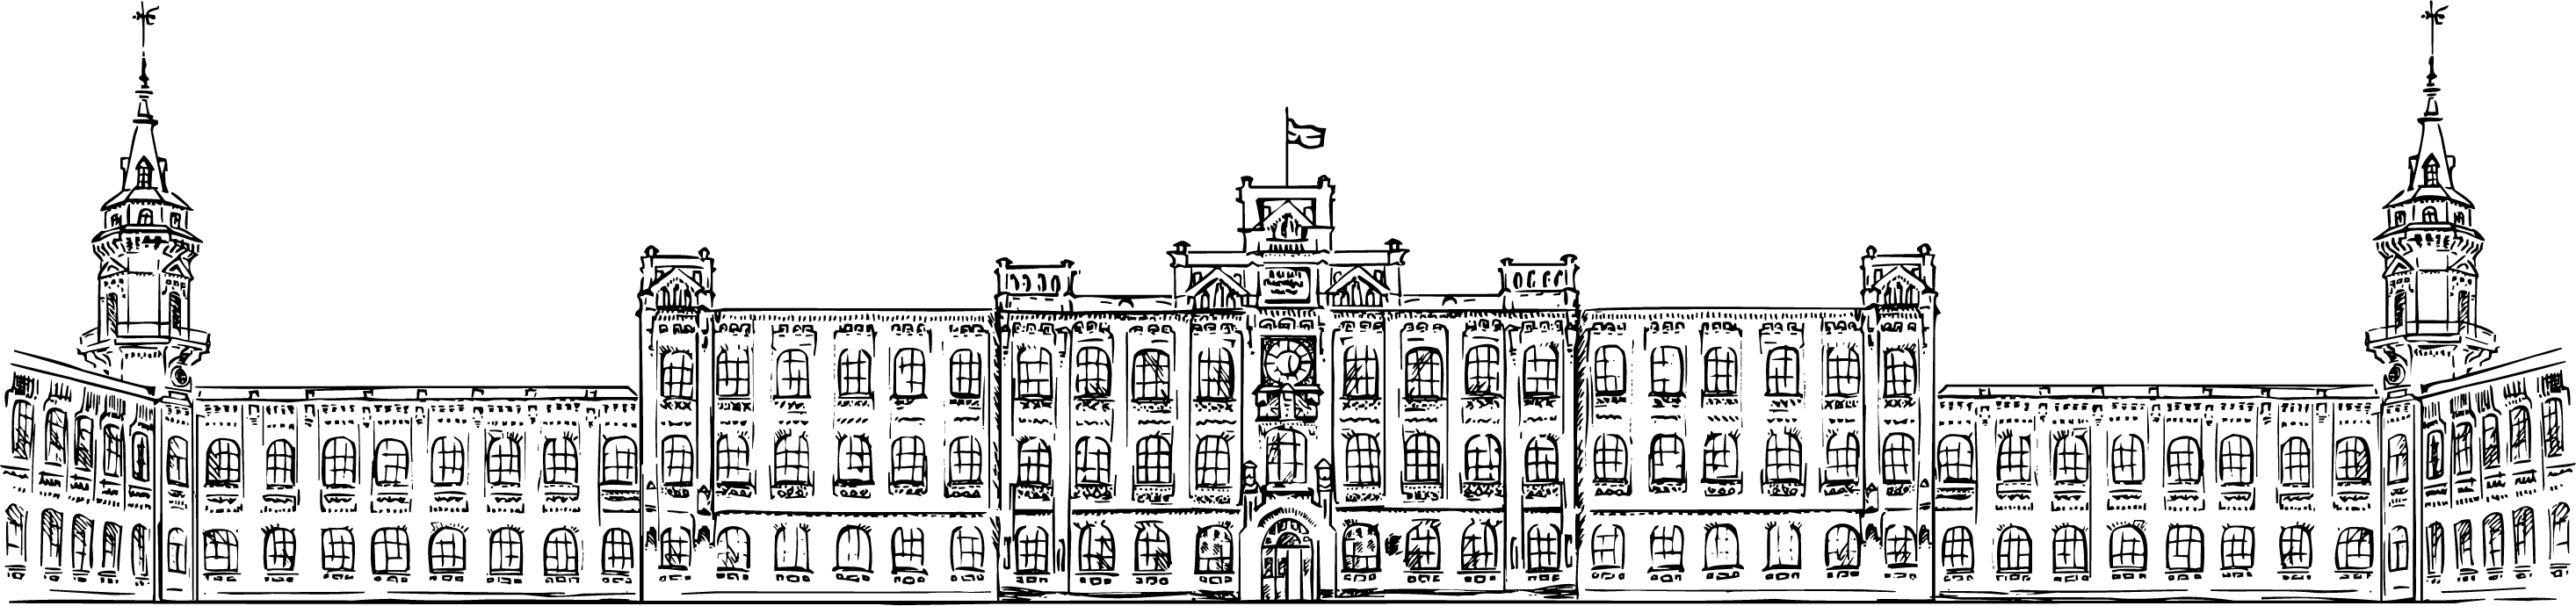
\includegraphics[width=0.7\textwidth]{../../../TITLES/letterhead.png}\end{center}

        \begin{center}
            \large Національний технічний університет України\\
            «Київський політехнічний інститут імені Ігоря Сікорського»\\[1em]
            Факультет інформатики та обчислювальної техніки\\
            Кафедра обчислювальної техніки
        \end{center}

        \vfill

        \begin{center}
            \textbf{\LARGE Практична електроніка}\\[2em]
            \textbf{\Large Лабораторна робота №3}\\[1em]
            «Діодні та транзисторні ключі»
        \end{center}

        \vfill

        \begin{flushright}
            Виконав: студент 2 курсу ФІОТ, гр. ІО-41\\
            \textit{Давидчук А.~М.}\\[1em]
            Перевірив: \textit{Гайдай А.~Р.}
        \end{flushright}

        \vfill

        \begin{center}Київ --- 2025\end{center}

    \end{titlepage}

    % Основний документ:

    \setlength{\parindent}{0em}

    \textbf{\underline{Тема:}} «Діодні та транзисторні ключі».

    \vspace{1em}

    \textbf{\underline{Мета:}} Дослідити принцип дії, основні властивості та характеристики діодних
та транзисторних ключів (ДК та ТК). Ознайомитись із основними параметрами цих
пристроїв та областю їх застосування.

    \begin{center} \textbf{\Large Практична частина} \end{center}

    Мiй порядковий номер у списку: 6. Звiдси визначу, що $A = 6$.

    \begin{center} \textbf{\large Аналіз схеми №1: Послідовний діодний ключ} \end{center}

    \setlength{\parindent}{1.5em}

    Робота всіх діодних ключів визначається станом діода: відкритий або
    закритий. Якщо потенціал анода більш додатний (менш від'ємний) ніж потенціал
    катода, то діод відкритий. В іншому випадку діод закритий.

    Побудуємо схему із послідовним діодним ключем:

    \begin{figure}[h!]

        \renewcommand{\thefigure}{\arabic{figure}} % робимо "3.1", "3.2" і т.д.

        \centering
        \includegraphics[width=0.7\textwidth]{scheme1.pdf}
        \caption{Схема послідовного діодного ключа}

    \end{figure}

    Та наведемо передатну характеристику (б) та часові діаграми роботи (а) діодного ключа, схему якого наведено на Рис. 1:

    \begin{figure}[h!]
        \centering

        \begin{subfigure}{0.48\textwidth}
            \centering
            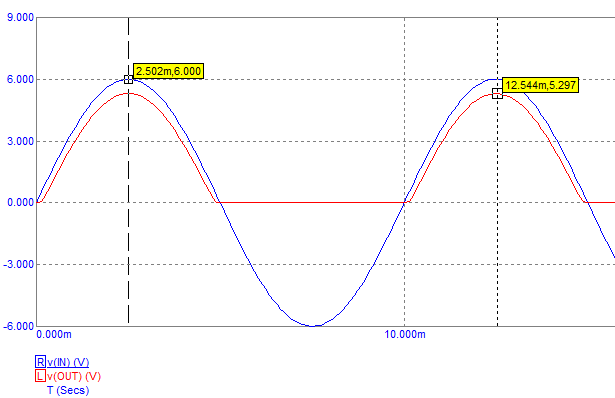
\includegraphics[width=\linewidth]{graph1-1.png}
            \caption{Часові діаграми роботи діодного ключа}
        \end{subfigure}\hfill
        \begin{subfigure}{0.48\textwidth}
            \centering
            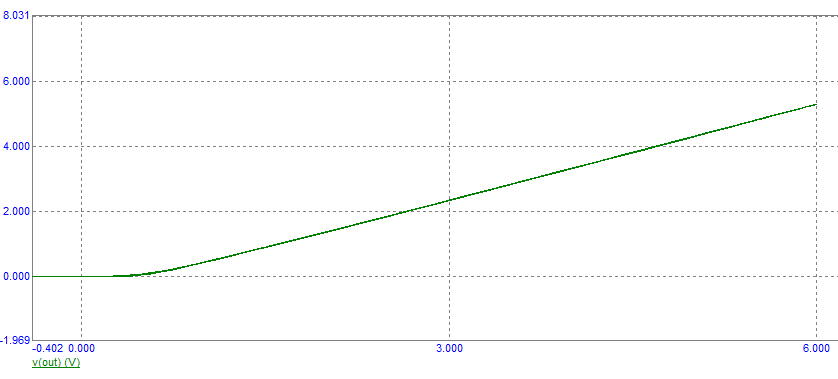
\includegraphics[width=\linewidth]{graph1-2.png}
            \caption{Передатна характеристика}
        \end{subfigure}

        \caption{Часові діаграми та передатна характеристика діодного ключа}
    \end{figure}

    Різниця між вхідною та вихідною напругами на рис. 25(вгорі) пояснюється
    тим, що послідовний діодний ключ пропускає тільки додатні напруги, а при
    від'ємних закривається.
    Деяка різниця між амплітудою вхідної та вихідної напруг для відкритого
    стану ключа зумовлена наявністю невеликого падіння напруги на відкритому діоді.
    Амплітуда графіка залежить від значення $A$, яку вказано в параметрах схеми (тут $A = 6$ В).

    \newpage

    \begin{center} \textbf{\large Аналіз схеми №2: Послідовний діодний ключ зі зміщенням} \end{center}

    Побудуємо таку схему:

    \begin{figure}[h!]

        \renewcommand{\thefigure}{\arabic{figure}} % робимо "3.1", "3.2" і т.д.

        \centering
        \includegraphics[width=0.7\textwidth]{scheme2.pdf}
        \caption{Схема послідовного діодного ключа зі зміщенням}

    \end{figure}

    Та наведемо передатну характеристику (б) та часові діаграми роботи (а) діодного ключа зі зміщенням:

    \begin{figure}[h!]
        \centering

        \begin{subfigure}{0.48\textwidth}
            \centering
            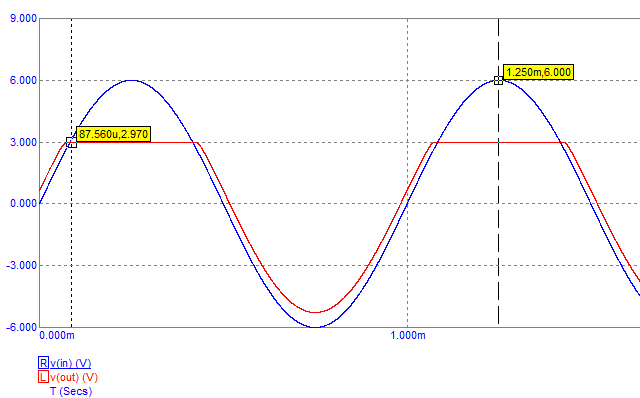
\includegraphics[width=\linewidth]{graph2-1.png}
            \caption{Часові діаграми роботи діодного ключа}
        \end{subfigure}\vfill
        \begin{subfigure}{0.9\textwidth}
            \centering
            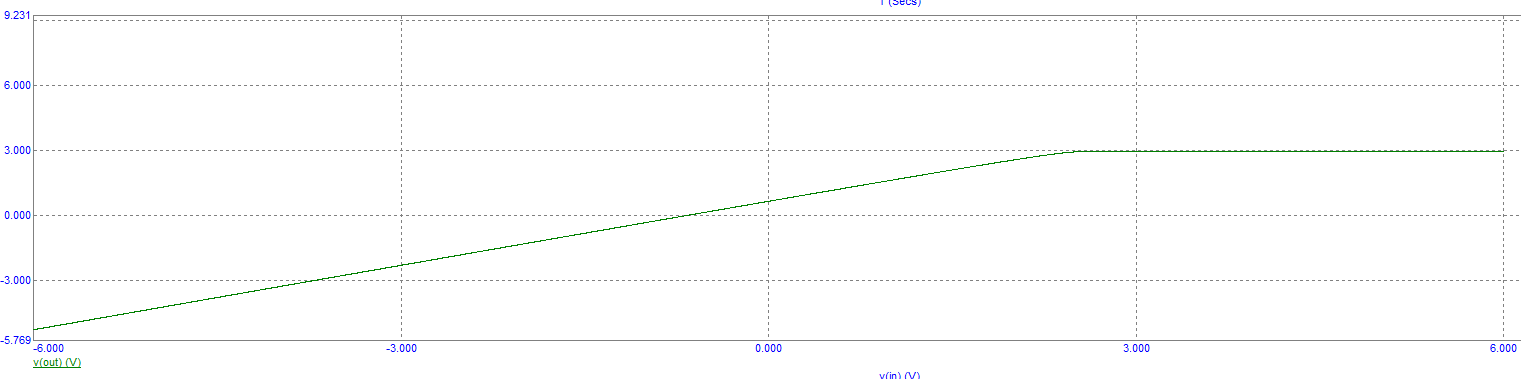
\includegraphics[width=\linewidth]{graph2-2.png}
            \caption{Передатна характеристика}
        \end{subfigure}

        \caption{Часові діаграми та передатна характеристика діодного ключа}
    \end{figure}

    На схемі наявна напруга зсуву $E_{\text{зс}} = 3$ B, через що діодний ключ закривається
    за додатною вхідною напругою $3$ В та з виходу знімається напруга $U_2 = 3$ В.

    \newpage

    \begin{center} \textbf{\large Аналіз схеми №3: Паралельний діодний ключ} \end{center}

    Побудуємо схему паралельного діодного ключа:

    \begin{figure}[h!]

        \renewcommand{\thefigure}{\arabic{figure}} % робимо "3.1", "3.2" і т.д.

        \centering
        \includegraphics[width=0.7\textwidth]{scheme3.pdf}
        \caption{Схема паралельного діодного ключа}

    \end{figure}

    Та наведемо передатну характеристику (б) та часові діаграми роботи (а) паралельного діодного ключа:

    \begin{figure}[h!]
        \centering

        \begin{subfigure}{0.48\textwidth}
            \centering
            
\includegraphics[width=\linewidth]{graph3-1.png}
            \caption{Часові діаграми роботи діодного ключа}
        \end{subfigure}\vfill
        \begin{subfigure}{0.9\textwidth}
            \centering
            
\includegraphics[width=\linewidth]{graph3-2.png}
            \caption{Передатна характеристика}
        \end{subfigure}

        \caption{Часові діаграми та передатна характеристика діодного ключа}
    \end{figure}

    Під час подачі на вхід ключа додатної напруги діод відкривається і напруга на ньому, а, отже, на виході близька до нуля.

    У разі надходження від'ємної вхідної напруги діод закривається і напруга на виході стає рівною напрузі на вході.

    \newpage

    \begin{center} \textbf{\large Аналіз схеми №4: Паралельний діодний ключ зі зміщенням} \end{center}

    Побудуємо схему паралельного діодного ключа зі зміщенням:

    \begin{figure}[h!]

        \renewcommand{\thefigure}{\arabic{figure}} % робимо "3.1", "3.2" і т.д.

        \centering
        \includegraphics[width=0.7\textwidth]{scheme4.pdf}
        \caption{Схема паралельного діодного ключа зі зміщенням}

    \end{figure}

    Та наведемо передатну характеристику (б) та часові діаграми роботи (а) паралельного діодного ключа зі зміщенням:

    \begin{figure}[h!]
        \centering

        \begin{subfigure}{0.48\textwidth}
            \centering
            
\includegraphics[width=\linewidth]{graph4-1.png}
            \caption{Часові діаграми роботи діодного ключа}
        \end{subfigure}\vfill
        \begin{subfigure}{0.9\textwidth}
            \centering
            
\includegraphics[width=\linewidth]{graph4-2.png}
            \caption{Передатна характеристика}
        \end{subfigure}

        \caption{Часові діаграми та передатна характеристика діодного ключа}
    \end{figure}

    Вид передатної характеристики пояснюється наступним чином: вона така ж
    сама, як на рис. 6 (паралельного ключа без зміщення), але перегорнута на $180^\circ$ через зворотне включення діода та
    піднята вгору на величину напруги зсуву $E_{\text{зс}}$, яка дорівнює $5$ В.

    \newpage

    \begin{center} \textbf{\large Аналіз схеми №5: Транзисторний ключ на базі n-p-n-транзистора під час подачі на вхід різнополярних імпульсів} \end{center}

    Побудуємо схему транзисторного ключа на базі n-p-n-транзистора під час подачі на вхід різнополярних імпульсів:

    \begin{figure}[h!]

        \renewcommand{\thefigure}{\arabic{figure}} % робимо "3.1", "3.2" і т.д.

        \centering
        \includegraphics[width=0.65\textwidth]{scheme5.pdf}
        \caption{\centering Схема транзисторного ключа на базі n-p-n-транзистора у разі подачі на
вхід різнополярних імпульсів}

    \end{figure}

    Та наведемо часові діаграми роботи (а, б) транзисторного ключа на базі n-p-n-транзистора під час подачі на вхід різнополярних імпульсів:

    \begin{figure}[h!]
        \centering

        \begin{subfigure}{0.56\textwidth}
            \centering
            
\includegraphics[width=\linewidth]{graph5-1.png}
            \caption{}
        \end{subfigure}\vfill
        \begin{subfigure}{0.56\textwidth}
            \centering
            
\includegraphics[width=\linewidth]{graph5-2.png}
            \caption{}
        \end{subfigure}

        \caption{Часові діаграми роботи транзисторного ключа}
    \end{figure}

    Вигляд характеристик, які наведено на рис. 10, пов'язаний з часовими діаграмами роботи транзисторного ключа у динамічному режимі (рис. 11):

    \begin{figure}[h!]

        \renewcommand{\thefigure}{\arabic{figure}} % робимо "3.1", "3.2" і т.д.

        \centering
        
\includegraphics[width=1.0\textwidth]{graph5-3.png}
        \caption{Часові діаграми роботи ТК}

    \end{figure}

    \newpage

    \begin{center} \textbf{\large Аналіз схеми №6: Транзисторний ключ на базі n-p-n-транзистора
включеного за схемою із спільним емітером з прискорюючим конденсатором
та без нього} \end{center}

    Побудуємо схему транзисторного ключа на базі n-p-n-транзистора
    включеного за схемою із спільним емітером з прискорюючим конденсатором
    та без нього:

    \begin{figure}[h!]

        \renewcommand{\thefigure}{\arabic{figure}} % робимо "3.1", "3.2" і т.д.

        \centering
        \includegraphics[width=0.9\textwidth]{scheme6.pdf}
        \caption{\centering Схема транзисторного ключа на базі n-p-n-транзистора, який включено
за схемою із спільним емітером з прискорюючим конденсатором та без нього}

    \end{figure}

    Та наведемо часові діаграми роботи (а, б) транзисторного ключа на базі на базі n-p-n-транзистора
    включеного за схемою із спільним емітером з прискорюючим конденсатором
    та без нього

    \begin{figure}[h!]
        \centering

        \begin{subfigure}{1.0\textwidth}
            \centering
            
\includegraphics[width=\linewidth]{graph6-1.png}
            \caption{}
        \end{subfigure}\vfill
        \begin{subfigure}{1.0\textwidth}
            \centering
            
\includegraphics[width=\linewidth]{graph6-2.png}
            \caption{}
        \end{subfigure}

        \caption{\centering Часові діаграми роботи транзисторного ключа із спільним емітером з прискорюючим конденсатором
    та без нього}
    \end{figure}

    На цьому рисунку зроблено порівняння характеристик вихідних сигналів для
    транзисторних ключів з прискорюючим конденсатором і без нього. Як видно з
    графіка, схема з прискорюючим конденсатором забезпечує більшу швидкодію
    транзисторного ключа (на графіку це видно по тому, що перехід від одного стану
    ТК до іншого став значно стрімкішим).

    \newpage

    На графіку б) видно, що транзисторний ключ з прискорюючим
    конденсатором забезпечує форму базового струму близьку до ідеальної:

    \begin{figure}[h!]

        \renewcommand{\thefigure}{\arabic{figure}} % робимо "3.1", "3.2" і т.д.

        \centering
        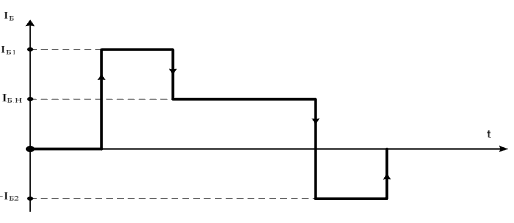
\includegraphics[width=0.65\textwidth]{graph6-3.png}
        \caption{Оптимальна форма вхідного базового струму ТК}

    \end{figure}

    Розглянемо роботу даної схеми детальніше. У початковий момент часу (коли
    ще не було керувального вхідного імпульсу) транзистор буде закритий (це
    забезпечується невеликим від'ємним потенціалом від батареї $E_{\text{б}}$ ($V3$)), тобто вихідна
    напруга буде приблизно дорівнювати $E_{\text{к}}$. Під час надходження керувального
    сигналу значення струму бази буде визначатися лише резистором $R4$ та амплітудою
    керувального сигналу, оскільки в початковий момент часу подачі керувального
    імпульсу заряд на конденсаторі дорівнює нулю, резистор $R1$ буде закорочений. У
    цьому разі ступінь насичення
    
    \[
    S = \frac{I_{\text{б}}}{I_{\text{бн}}}
    \]

    буде значно більшою одиниці, що
    прискорює відкривання ключа. Далі в міру того, як конденсатор буде
    заряджатися, струм бази буде зменшуватися за експоненціальним законом до
    сталого значення приблизно рівного:

    \[
    \frac{U1}{R4 + R1} - \frac{V3}{R5}
    \]

    Але оскільки другий
    доданок набагато менший першого, ним можна знехтувати. У цьому разі ступінь
    насичення $S$ буде близькою до одиниці.

    Після припинення подачі імпульсу відбудеться різкий стрибок струму бази у
    зворотному напрямку (це пов'язано з накопиченням неосновних зарядів в базі),
    відбудеться перезаряд конденсатора, за рахунок чого закоротиться резистор $R1$, що
    призведе до більш швидкого закриття транзистора, тобто меншому часу
    розсмоктування.

    Аналіз часових діаграм роботи транзисторного ключа показує, що процес перемикання складається з кількох послідовних етапів, кожен з яких характеризується певним часовим інтервалом.

    У початковому стані ($0 \div t_1$) транзистор закритий, обидва переходи непровідні, і вихідна напруга $U_{\text{вих}}$ велика.
    Після моменту $t_1$ (інтервал $t_1 \div t_2$) під дією позитивного вхідного сигналу починається процес відкривання транзистора. Робоча точка переміщується в область насичення, але це відбувається не миттєво, а протягом часу $\Delta t = t_2 - t_1$, який визначає тривалість фронту.
    У проміжку $t_2 \div t_3$ транзистор перебуває у стані насичення — він повністю відкритий, і вихідна напруга має мінімальне значення.
    Після зняття вхідного сигналу ($t_3 \div t_4$) починається процес закривання: відбувається розсмоктування надлишкового заряду бази, і напруга на виході зростає.
    Інтервал $\Delta t' = t_4 - t_3$ характеризує тривалість спаду.
    Після моменту $t_4$ транзистор повертається в початковий (закритий) стан.

    \newpage

    \begin{center} \textbf{\large Аналіз схеми №7: Транзисторний ключ на базі n-p-n-транзистора відкритого у
початковому стані, який включено за схемою із спільним емітером} \end{center}

    Нижче наведено схему транзисторного ключа на базі n-p-n-транзистора, який
    відкритий у початковому стані та включений за схемою із спільним емітером:

    \begin{figure}[h!]

        \renewcommand{\thefigure}{\arabic{figure}} % робимо "3.1", "3.2" і т.д.

        \centering
        \includegraphics[width=0.5\textwidth]{scheme7.pdf}
        \caption{\centering Схема транзисторного ключа на базі n-p-n-транзистора відкритого
у початковому стані, який включено за схемою із спільним емітером}

    \end{figure}

    Та наведемо часові діаграми роботи цього транзисторного ключа:

    \begin{figure}[h!]

        \renewcommand{\thefigure}{\arabic{figure}} % робимо "3.1", "3.2" і т.д.

        \centering
        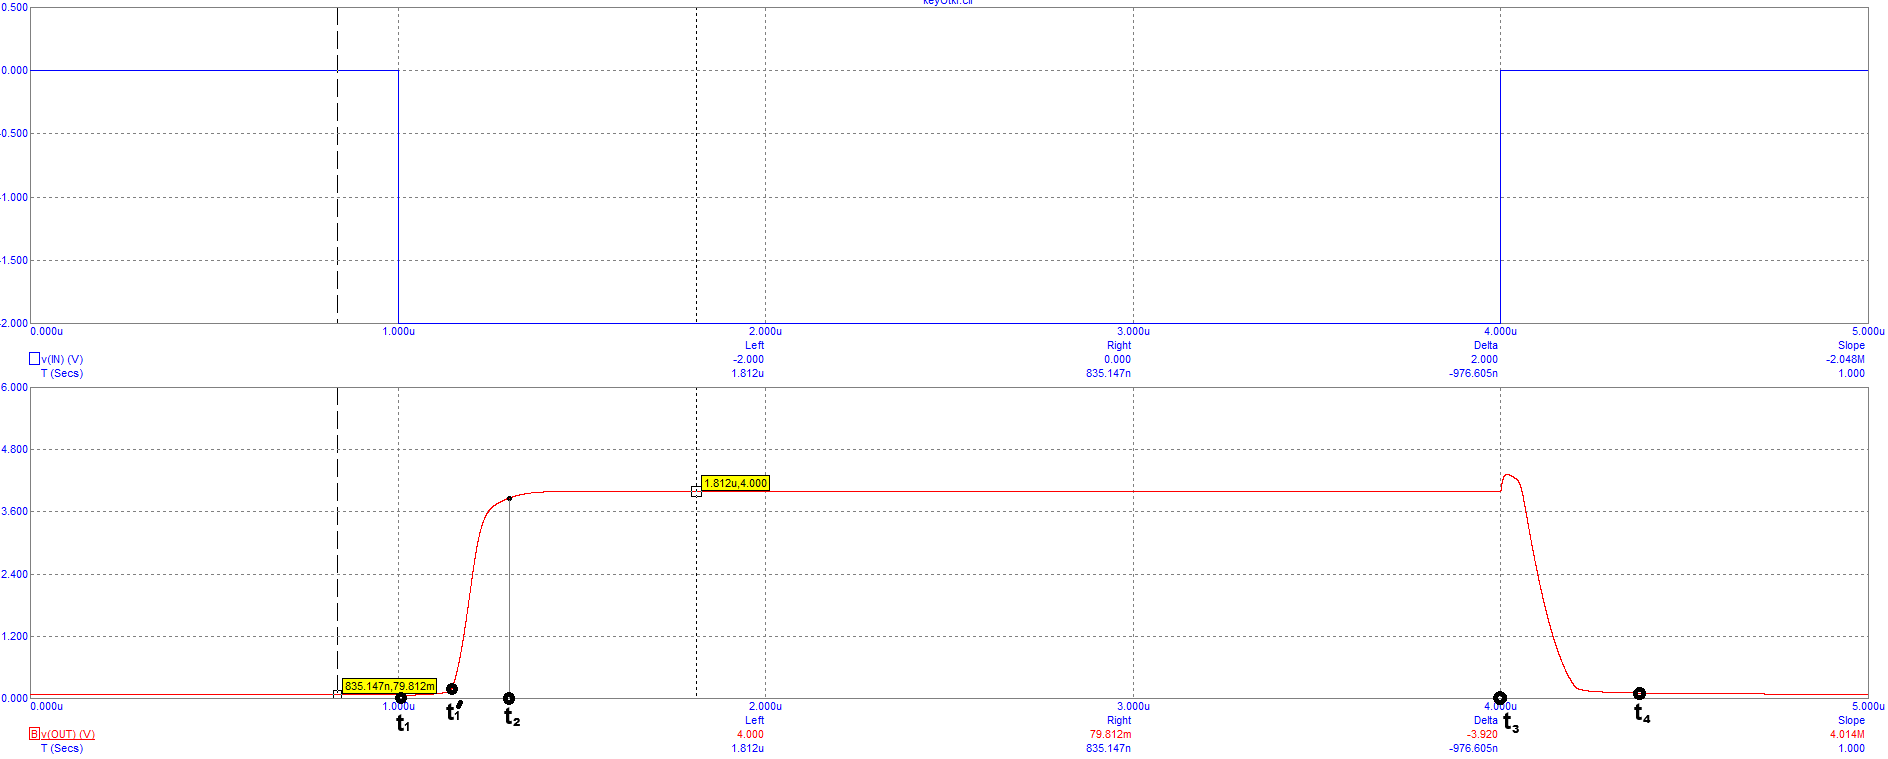
\includegraphics[width=1.0\textwidth]{graph7.png}
        \caption{\centering Часові діаграми роботи транзисторного ключа на базі n-p-nтранзистора,
відкритого у початковому стані, який включено за схемою із спільним емітером}

    \end{figure}

    На цьому рисунку ми бачимо залежність вхідної та вихідної напруг від часу
    транзисторного ключа на базі n-p-n-транзистора відкритого у початковому стані,
    який включено за схемою із спільним емітером (синя лінія – вхідна напруга,
    червона – вихідна).

    Інтервал $0 \div t_1$: $U_{\text{вх}} = 0$, ключ відкритий тому, що на базі p-типу присутній
    додатний потенціал від джерела $V2$ ($E_{\text{к}}$). З виходу знімається невелика напруга.

    Інтервал $t_1 \div t_1'$: після подачі на вхід схеми напруги від'ємної полярності,
    транзистор закривається, але це відбувається не миттєво, а лише через час $\Delta t = t_1' - t1$ -- час розсмоктування надлишкового заряду в базі транзистора.
    Наявність цієї затримки говорить про те, що у відкритому стані струм бази був більшим за струм бази
    насичення: $I_{\text{б}} > I_{\text{бн}}$.

    Інтервал $t_1' \div t_2$: після закінчення часу розсмоктування ключ закривається, але
    це відбувається лише через час $\Delta t = t_2 - t_1'$, який називають тривалістю фронта.

    Інтервал $t_2 \div t_3$: ТК закритий, напруга на виході схеми максимальна і
    дорівнює: $U_{\text{вих}} = E_{\text{к}} - I_{\text{к0}} \cdot R_{\text{к}}$.

    Інтервал $t_3 \div t_4$: у разі відключення вхідного сигналу ($U_{\text{вх}} = 0$) після
    перебування ТК у закритому стані, необхідно час $t = t_4 - t_3$. За цей час переходи
    транзистора відкриваються.

    Інтервал $t > t_4$: транзистор відкритий, і ТК перебуває в своєму початковому
    стані.

    \begin{center} \textbf{\large Аналіз схеми №8: Транзисторний ключ на базі n-p-n-транзистора закритого у
початковому стані, який включено за схемою із спільним емітером} \end{center}

    Нижче наведено схему транзисторного ключа на базі n-p-n-транзистора
закритого у початковому стані, який включено за схемою із спільним емітером:

    \begin{figure}[h!]

        \renewcommand{\thefigure}{\arabic{figure}} % робимо "3.1", "3.2" і т.д.

        \centering
        \includegraphics[width=0.6\textwidth]{scheme8.pdf}
        \caption{\centering Схема транзисторного ключа на базі n-p-n-транзистора закритого у
початковому стані, який включено за схемою із спільним емітером}

    \end{figure}

    Та наведемо часову діаграму роботи цього транзисторного ключа, схему якого наведено на рис. 17:

    \begin{figure}[h!]

        \renewcommand{\thefigure}{\arabic{figure}} % робимо "3.1", "3.2" і т.д.

        \centering
        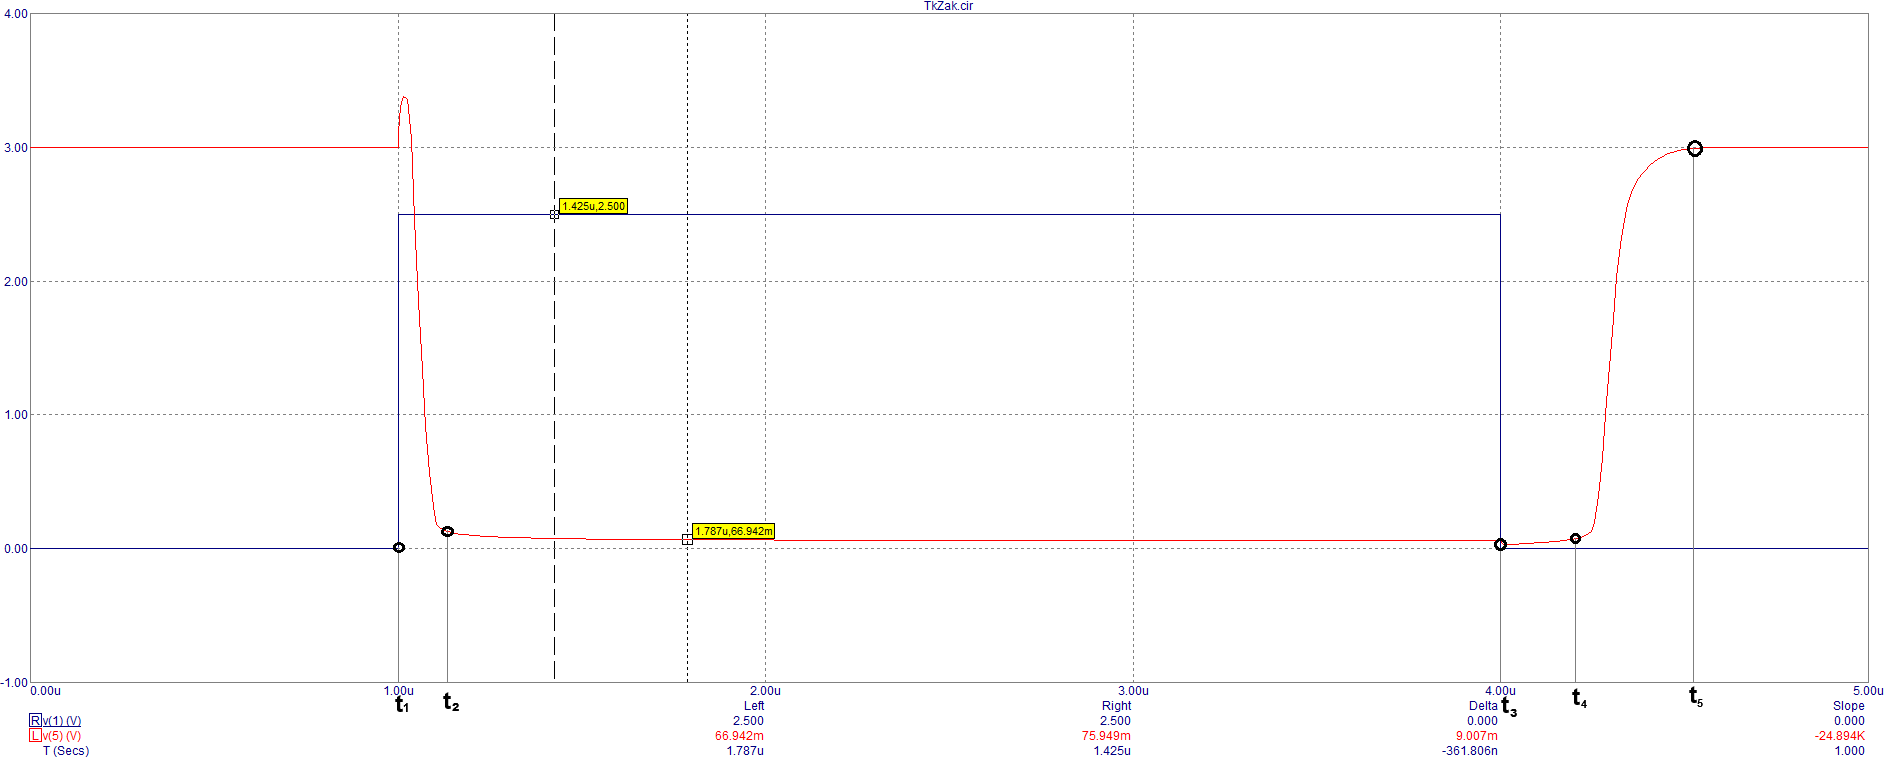
\includegraphics[width=0.8\textwidth]{graph8.png}
        \caption{\centering Часові діаграми роботи транзисторного ключа на базі n-p-n-транзистора,
закритого у початковому стані, який включено за схемою із спільним емітером}

    \end{figure}

    На цьому рисунку ми бачимо залежність вхідної та вихідної напруг від часу
    закритого транзисторного ключа на базі n-p-n-транзистора, який включено за
    схемою із спільним емітером (синя лінія – вхідна напруга, червона – вихідна).

    Інтервал $0 \div t_1$: $U_{\text{вх}} = 0$ В, але через наявність джерела $Е_1$ потенціал бази
    р-типу транзистора від'ємний, а оскільки на колектор подається «плюс» і емітер
    заземлений, обидва переходи транзистора n-p-n-типу закриті, і напруга колектор-
    емітер ($U_{\text{вих}}$) велика.

    Інтервал $t_1 \div t_2$: після подачі на вхід схеми напруги додатної полярності,
    достатньої для відмикання p-n-переходів, транзистор відкривається, але
    відбувається це не миттєво, а лише через час $\Delta t = t_2 - t_1$, який називають тривалістю
    фронту.

    Інтервал $t_2 \div t_3$: ТК відкритий, напруга на виході схеми дорівнює падінню
    напруг на відкритих переходах і є невеликою.

    Інтервал $t_3 \div t_4$: у разі відключення вхідного сигналу ($U_{\text{вх}} = 0$) для
    розсмоктування надлишкового заряду, який накопичився в базі за час перебування
    ТК у відкритому стані, необхідно час $\Delta t = t_4 - t_3$. За цей час переходи транзистора
    починають закриватися. Наявність цього $\Delta t$ говорить про те, що струм бази у
    відкритому стані був значно більше струму бази насичення ($I_{\text{б}} >> I_{\text{бн}}$).

    Інтервал $t_4\dots t_5$ -- формування заднього фронту.

    Інтервал $t > t_5$: транзистор закритий і ТК знаходиться в своєму початковому
    стані.

    \begin{center} \textbf{\large Аналіз схеми №9: Транзисторний ключ на базі польового транзистора} \end{center}

    Нижче наведено схему транзисторного ключа на базі польового транзистора МОН-типу:

    \begin{figure}[h!]

        \renewcommand{\thefigure}{\arabic{figure}} % робимо "3.1", "3.2" і т.д.

        \centering
        \includegraphics[width=0.6\textwidth]{scheme9-1.pdf}
        \caption{\centering Схема транзисторного ключа на базі польового транзистора МОН-типу з n-
каналом, який індукується}

    \end{figure}

    На рис. 19, який наведено вище, в якості польового транзистору обрано МОН-транзистор із індукованим каналом n-типу. У МОН-ПТ із каналом, що індукується,
    на відміну від ПТ з p-n-переходами канал між областями витоку і стоку при виготовленні транзистора технологічно не створюється (відсутній):

    \begin{figure}[h!]

        \renewcommand{\thefigure}{\arabic{figure}} % робимо "3.1", "3.2" і т.д.

        \centering
        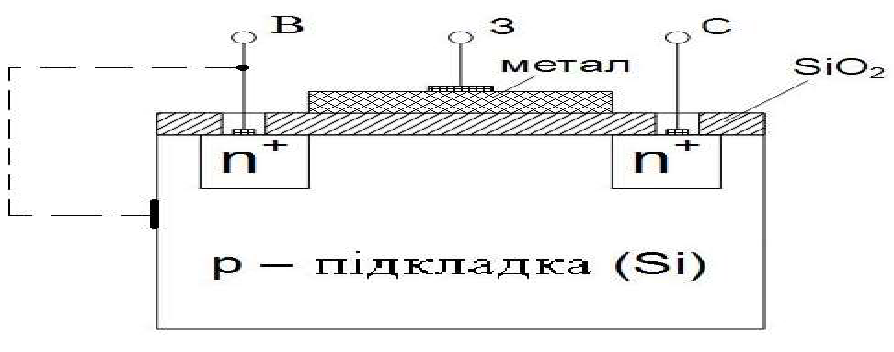
\includegraphics[width=0.5\textwidth]{graph9-1.png}
        \caption{Спрощена структура МДН ПТ із каналом n-типу, що індукується}

    \end{figure}

    \newpage

    Канал індукується за рахунок явища інверсії, яке виникає у системі метал-
    діелектрик-напівпровідник. У разі подачі на затвор напруги додатної полярності
    індукується канал n-типу, від'ємної полярності -- p-типу.

    Тобто МОН-ПТ із каналом, що індукується, керується напругою затвору лише
    одного знаку. На рис. 20 наведено структуру МОН-ПТ із каналом n-типу, що
    індукується, який керується додатною напругою на затворі. На рис. 21 зображено
    стоко-затворну і стокові характеристики такого транзистора.

    \begin{figure}[h!]
        \centering

        \begin{subfigure}{0.48\textwidth}
            \centering
            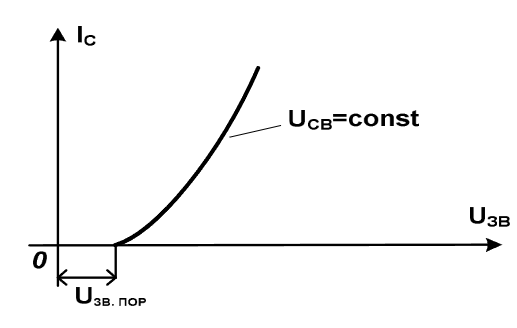
\includegraphics[width=\linewidth]{graph9-2.png}
            \caption{}
        \end{subfigure}\hfill
        \begin{subfigure}{0.48\textwidth}
            \centering
            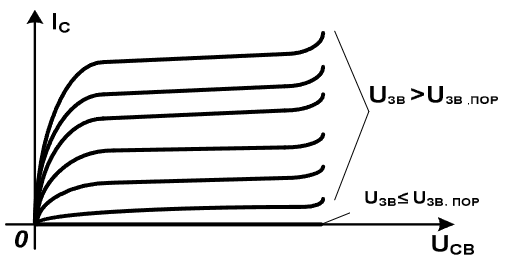
\includegraphics[width=\linewidth]{graph9-3.png}
            \caption{}
        \end{subfigure}

        \caption{\centering Статичні ВАХ МОН ПТ із n-каналом, що індукується:
а -- вхідні; б -- вихідні}
    \end{figure}

    Подібно до біполярних транзисторів ПТ можна включати в електричний
    ланцюг за однією з трьох схем: СВ – спільним витоком; СЗ -- спільним затвором і
    СС -- спільним стоком. Найчастіше застосовується схема включення ПТ із спільним
    витоком (рис. 19).

    На рис. 22 наведено часові діаграми роботи транзисторного ключа, схему
    якого наведено на рис. 19:

    \begin{figure}[h!]

        \renewcommand{\thefigure}{\arabic{figure}} % робимо "3.1", "3.2" і т.д.

        \centering
        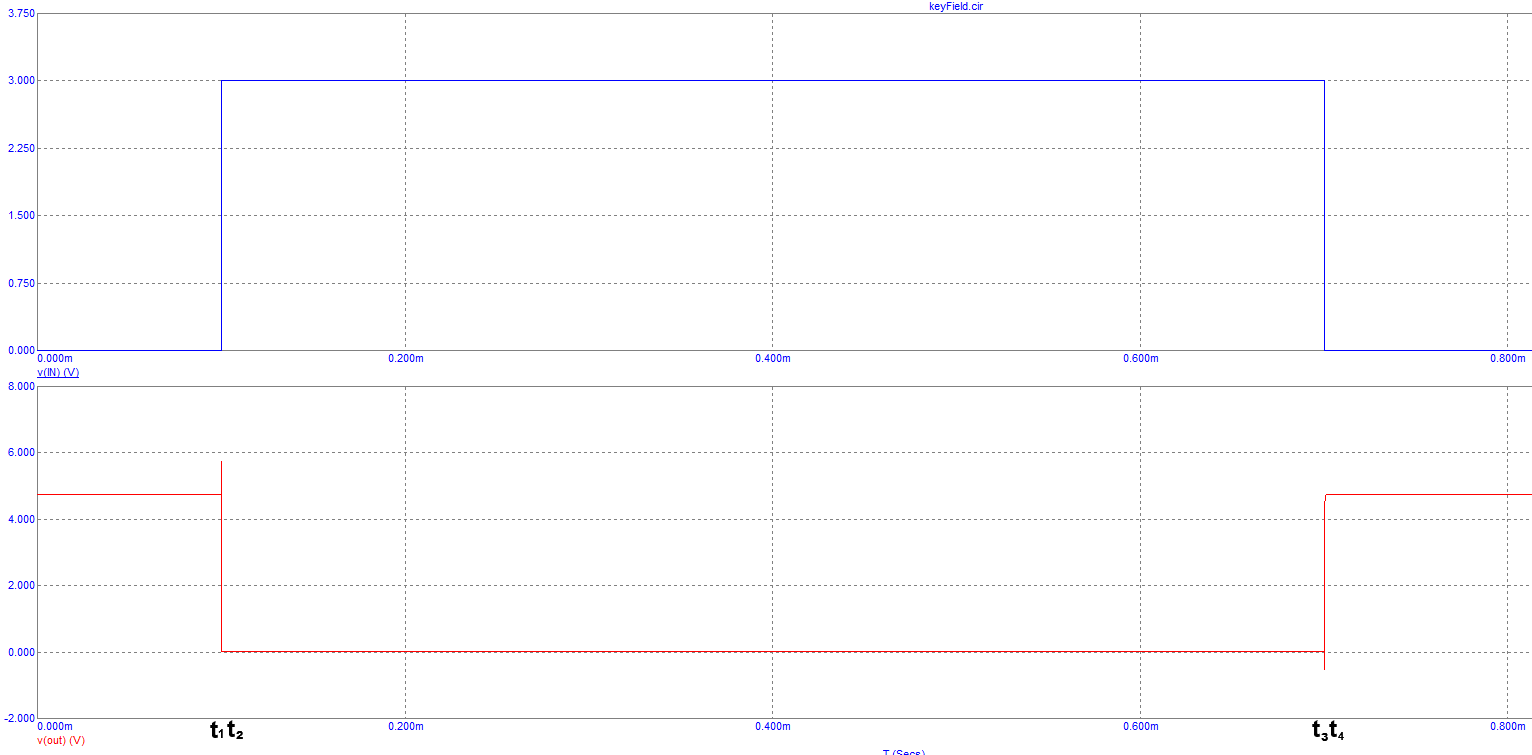
\includegraphics[width=0.6\textwidth]{graph9-4.png}
        \caption{Часові діаграми роботи ТК на польовому МОН-транзисторі}

    \end{figure}

    У вихідному стані, коли $U_{\text{вх}} = 0$ В, каналу, який проводить струм, в підкладці
    транзистора немає, тому ТК закритий. Це означає, що $I_{\text{с}} = I_{\text{в}} = 0$ і вся напруга джерела
    живлення $V2$ подається на вихід схеми: $U_{\text{вх}} = V2$. Такому стану схеми на графіку
    відповідає відрізок часу $t = 0 \div t_1$.

    Якщо на вхід схеми подавати напругу додатної полярності, то при певному її
    значенні через транзистор почне протікати струм.

    Це пояснюється тим, що в підкладці p-типу між витоком та стоком буде
    індукуватися канал (n-типу), який забезпечить електричне з'єднання електродів
    транзистора (вони також мають тип провідності -- n). Врешті ТК відкриється і $U_{\text{вих}}$,
    яке дорівнює падінню напруги на опорі каналу, в цьому випадку буде невеликим
    (близьким до нуля), що підтверджують наведені нижче графіки. Як видно, в момент
    відмикання ключа ($t = t_1$) $U_{\text{вих}}$ зменшується не миттєво.
    Це пов'язано з обмеженістю швидкості формування провідного каналу.

    Коли керувальна напруга $U_{\text{вх}}$ знову впаде до 0 (момент $t_3$), електрони у
    підкладці транзистора під дією дифузійного ефекту будуть рівномірно
    розподілятися за її об'ємом і канал поступово через деякий час зникне. ТК
    закриється, і вихідна напруга знову зросте до значення $V2$.

    Нижче наведено схему для зняття стоко-затворної характеристики
транзисторного ключа на базі польового МОН-транзистора:

    \begin{figure}[h!]

        \renewcommand{\thefigure}{\arabic{figure}} % робимо "3.1", "3.2" і т.д.

        \centering
        \includegraphics[width=0.4\textwidth]{scheme9-2.pdf}
        \caption{Схема для зняття стоко-затворної характеристики польового МОН-
транзистора}

    \end{figure}

    На рис. 24 наведено стоко-затворну характеристику польового МОН-транзистора:

    \begin{figure}[h!]

        \renewcommand{\thefigure}{\arabic{figure}} % робимо "3.1", "3.2" і т.д.

        \centering
        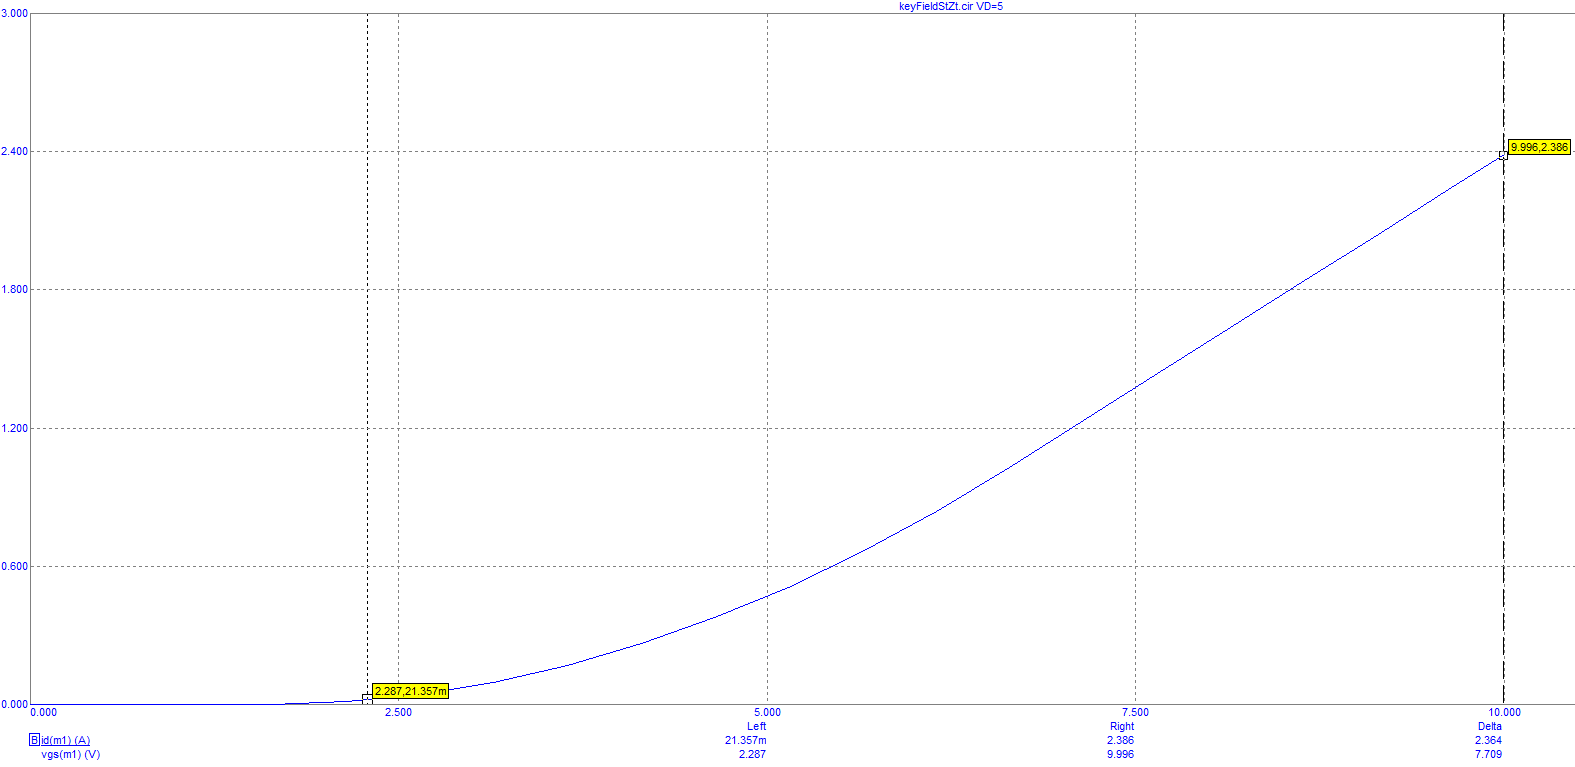
\includegraphics[width=0.9\textwidth]{graph9-5.png}
        \caption{Стоко-затворна характеристика польового МОН-транзистора}

    \end{figure}

    Ця стоко-затворна характеристика показує, що формування каналу
    починається, коли $U_{\text{вх}}$ досягає значення $U_{\text{пор}}$.

    Максимальне значення струму стоку в схемі на рис. 19 визначається
    резистором $R2$:

    \[
    I_{\text{c. max}} \approx \frac{V2}{R2}
    \]

    \newpage

    \begin{center} \textbf{\large Аналіз схеми №10: Транзисторний ключ на базі діода Шотткі} \end{center}

    Нижче наведено схему транзисторного ключа на базі діода Шотткі:

    \begin{figure}[h!]

        \renewcommand{\thefigure}{\arabic{figure}} % робимо "3.1", "3.2" і т.д.

        \centering
        \includegraphics[width=0.4\textwidth]{scheme10.pdf}
        \caption{Схема транзисторного ключа на базі діода Шоткі}

    \end{figure}

    На рис. 26 наведено часові діаграми роботи ТК на біполярному n-p-n-транзисторі без та з діодом Шотткі:

    \begin{figure}[h!]

        \renewcommand{\thefigure}{\arabic{figure}} % робимо "3.1", "3.2" і т.д.

        \centering
        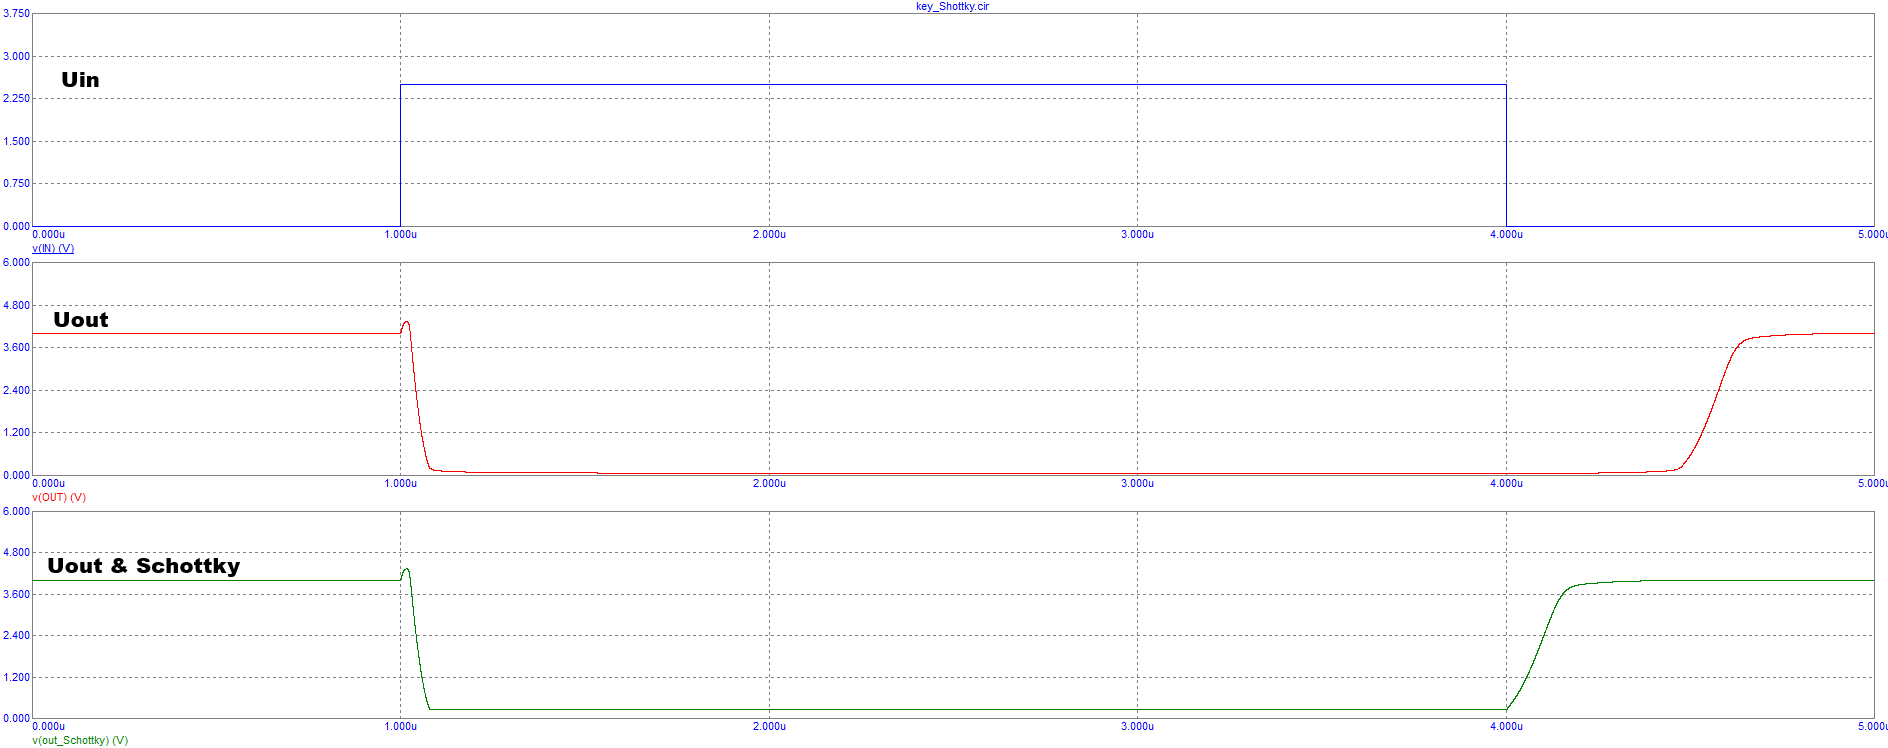
\includegraphics[width=0.9\textwidth]{graph10.png}
        \caption{\centering Часові діаграми роботи ТК на біполярному n-p-n-транзисторі без та з діодом
Шотткі}

    \end{figure}

    На вихідних характеристиках добре видно, що у разі подання на вхід
    додатного імпульсу обидва ТК змінюють стан (відкриваються) за однаковий час.
    Проте ТК на базі діода Шотткі більш швидко повертається у початковий стан
    (закривається) за рахунок меншого часу перехідного процесу.

    \vspace{1em}
    \setlength{\parindent}{0em}

    \textbf{\underline{Висновок:}} У ході виконання лабораторної роботи було досліджено принцип дії, властивості та часові характеристики діодних і транзисторних ключів. 
Проаналізовано роботу послідовних і паралельних діодних ключів, а також вплив напруги зміщення на форму передатних характеристик і часових діаграм. 
Встановлено, що діодні ключі пропускають сигнали лише певної полярності, а наявність напруги зміщення дозволяє зміщувати поріг спрацювання.

    \setlength{\parindent}{1.5em}

Дослідження транзисторних ключів показало, що процес перемикання не є миттєвим і складається з кількох послідовних етапів: відкривання, насичення та закривання транзистора. 
Кожен етап характеризується певними часовими інтервалами ($t_1$, $t_2$, $t_3$, $t_4$), які визначають фронти та спади сигналів. 
Тривалість цих інтервалів зумовлена ємнісними властивостями переходів, величиною струму бази та конструктивними особливостями схеми.

Показано, що застосування прискорюючого конденсатора сприяє зменшенню часу відкривання та закривання транзистора, підвищуючи його швидкодію. 
Використання діода Шотткі запобігає перенасиченню транзистора, скорочує час розсмоктування надлишкового заряду та забезпечує більш швидке повернення ключа у вихідний стан. 
Ключі на польових транзисторах, завдяки керуванню напругою й високому вхідному опору, мають ще більшу швидкодію й енергетичну ефективність, що робить їх придатними для сучасних цифрових схем.

Отже, експериментально підтверджено основні закономірності роботи діодних і транзисторних ключів, виявлено вплив додаткових елементів 
(напруги зміщення, прискорюючого конденсатора, діода Шотткі) на їх динамічні параметри. 
Отримані результати демонструють, що застосування таких елементів дає змогу значно підвищити швидкодію та надійність комутаційних схем на транзисторах.

\end{document}